\documentclass{report}

\usepackage[utf8]{inputenc}
\usepackage[T1]{fontenc}
\usepackage[francais]{babel}
\usepackage[textwidth = 400pt]{geometry}
\usepackage{url}
\usepackage{graphicx}
\usepackage{float}
\usepackage{longtable}
\usepackage{csvsimple}
\usepackage[table]{xcolor}
\usepackage{color}
\usepackage{lastpage}
\usepackage{fancyhdr}
\usepackage{appendix}



\begin{document}


\title {Projet de réalisation d'une IHM : OptiFret Lyon \\ Conception de l'IHM}
\author{Dragibus}
\maketitle


\newpage
~~\\
\textbf{Equipe Dragibus} : Hexanôme H4104 \\
Patrizia Peller\\
Mathis Paul\\
Sylvain Abadie\\
Quentin Coursodon\\
Pierre Turpin\\
Jean Marie Comets\\
Julien Rollet\\

~~\\
\textbf{Responsable Qualité} : Patrizia Peller\\
~~\\
\textbf{Gestion de Projet} : Julien Rollet\\


\newpage
\tableofcontents
\newpage


%-------------------DTU-------------------------%

\chapter{Description des Tâches de l'Utilisateur}

\paragraph{}
Pour cette première partie de la conception d'OptiFret, nous avons séparé l'équipe en deux groupes de travail :\\
Equipe A : Q Coursodon, M Paul, P Peller \\
Equipe B : P Turpin, S Abadie, JM Comets\\

L'Equipe A a travaillé sur : DDF \\

L'Equipe B a travaillé sur : MU / DPU / GPU \\

L’ensemble de l’équipe a travaillé sur : TTU / DF, DTU / DF, SPU \\


\section{Description des Domaines Fonctionnels}

\begin{tabular}{|c|c|l|}
\hline
D.1 & Administration des Systèmes informatiques& D.1.1 Maintenance\\
&&																							 D.1.2 Gestion utilisateurs\\
\hline
D.2 & Gestion des Ressources Humaines & D.2.1 Recrutement\\
&&																			D.2.2 Gestion du personnel\\
\hline
D.3 & Comptabilité & D.3.1 Gestion couts internes\\
&&									 D.3.2 Gestion salaires\\
&&									D3.3 Gestion factures clients\\
\hline
D.4 & Gestion des relations clientèles & D.4.1 Gestion SAV\\
&&																			D.4.2 Gestion contrats\\
\hline
D.5 &  Gestion des livraisons & D.5.1 Gestion des demandes de livraison\\
&&															D.5.2 Préparation et supervision des livraisons\\
&&															D.5.3 Réalisation des livraisons\\
\hline
\end{tabular}
~~\\
~~\\
D.1.1 Maintenance corrective et préventive permettant le bon fonctionnement du SI.\\
D.1.2 Création des utlisateurs, type d’utilisateur, gestion des droits.\\
~~\\
D.2.1 Ensemble des actions et démarche pour trouver sélectionner des candidats.\\
D.2.2 Gestion des congés, des abscences, formation continue.\\
~~\\
D.3.1 Gestion comptable de l’entreprise.\\
D.3.2 Gestion de la rémunération des employés.\\
D.3.3 Suivi des paiements par les clients.\\
~~\\
D.4.1 Prise en compte des plaintes des utilisateurs.\\
D.4.2 Démarchage des clients et négociation de contracts.\\
~~\\
D.5.1  Enregistrement des demandes de livraison, mise en relation du client et de l’entreprise de transport.\\
D.5.2 Génération des feuilles de routes, modification des feuilles de routes, suivi de l’états des livraisons en cours, des livreurs.\\
D.5.3 Transport des colis entre l'entrepôt du fournisseur et le client.\\

\paragraph{}

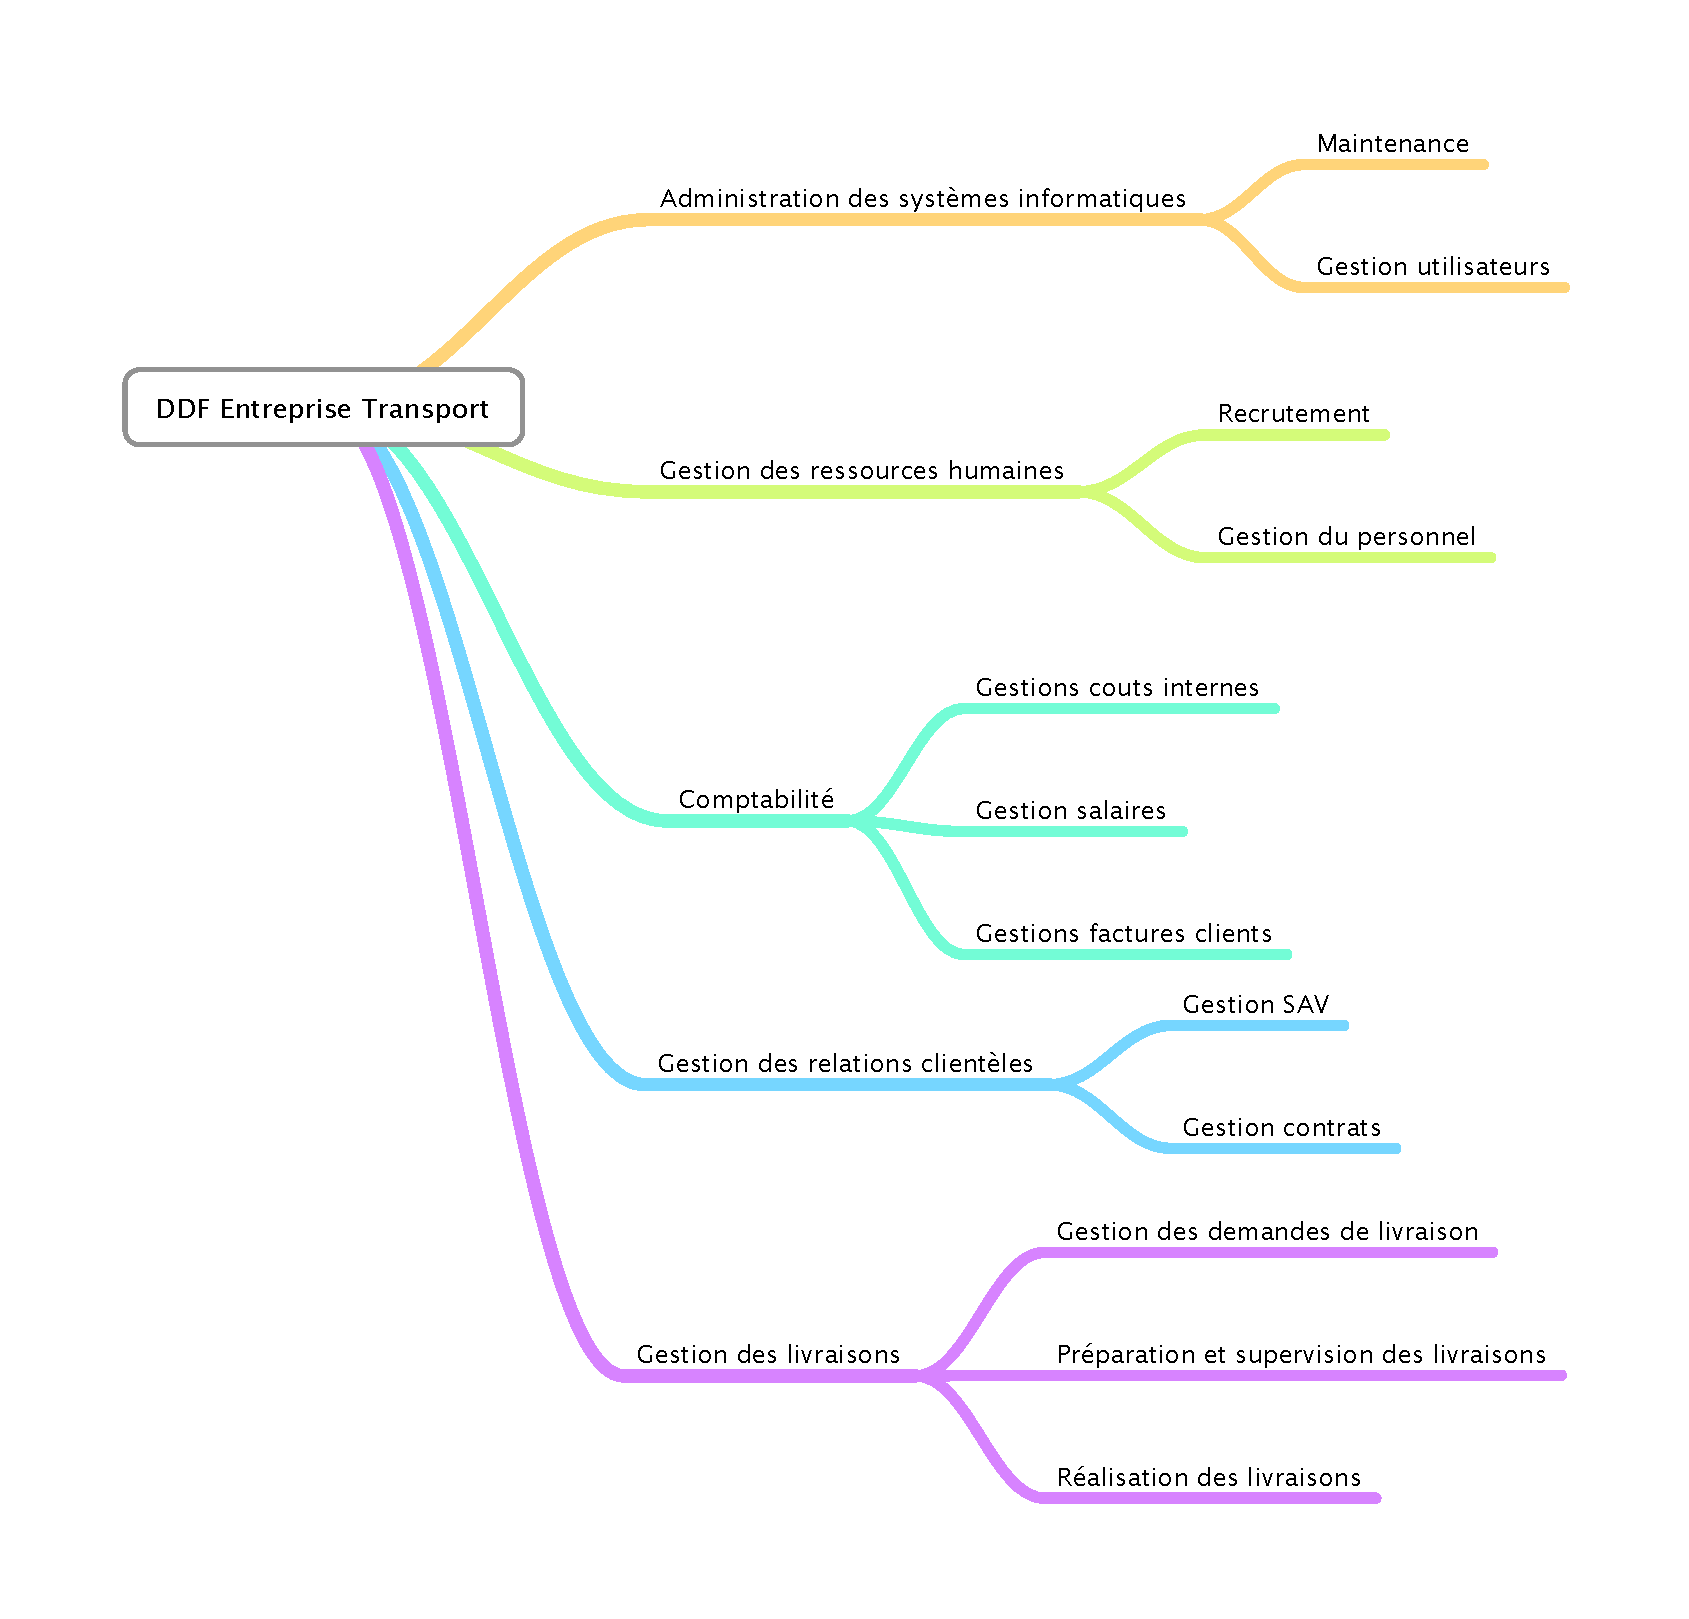
\includegraphics[scale = 0.4]{images/DDF.pdf}


\section{Modèle des Utilisateurs}

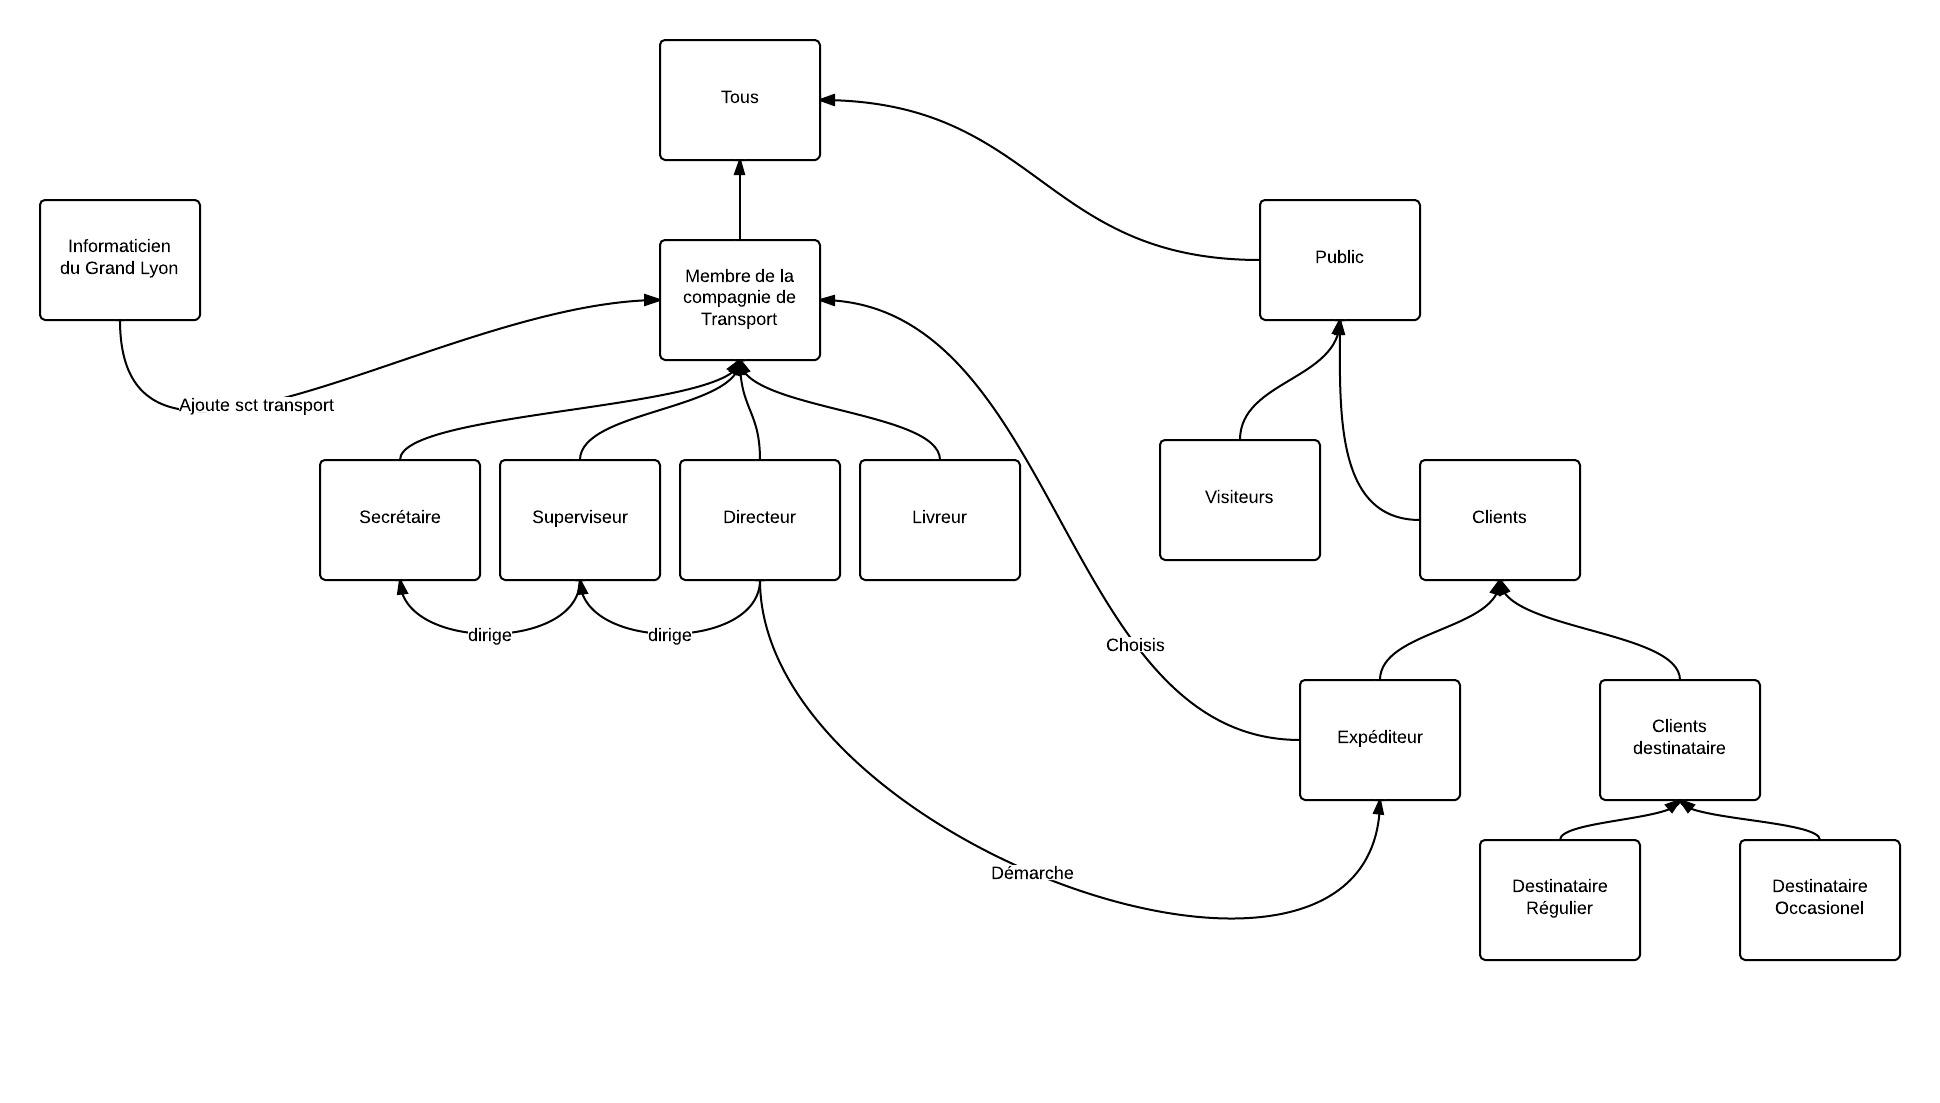
\includegraphics[scale = 0.3, angle=90]{images/MU.jpeg}


\section{Graphe d'héritage des Profils Utilisateurs}

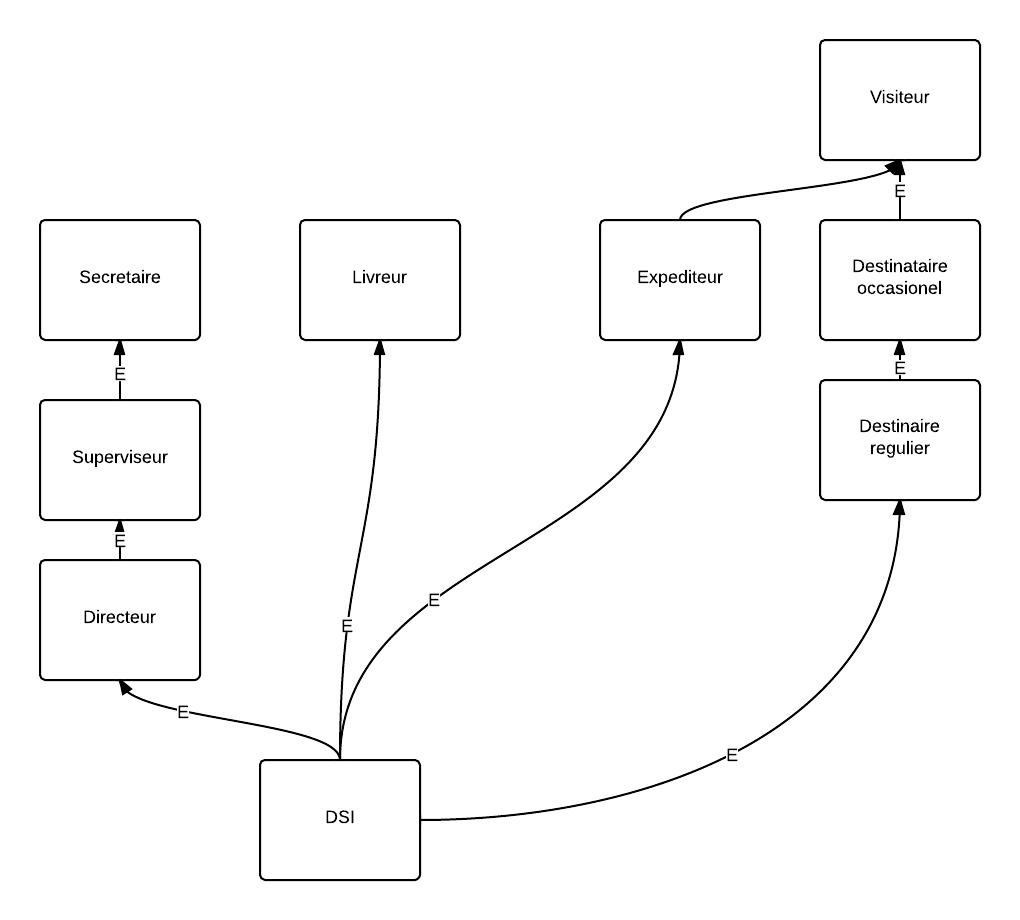
\includegraphics[scale = 0.25]{images/GPU.jpeg}

\section{Description des Profils Utilisateurs}

\begin{itemize}

\item{Directeur:} Directeur d’une entreprise de transport. Gère son entreprise en démarchant des clients ayant besoin d’expédier des marchandises (ex : amazon, fnac ...). Il dirige les superviseurs et les secrétaires et peut potentiellement les remplacer dans leurs tâches.\\ 

\item{Livreur :} CFP (contrat de formation professionnelle) de livreur, doit être détenteur d’un permis B (conduite de véhicule léger allant jusqu’à 3,5 tonnes). Il se doit d’être ponctuel et actif. Il doit également connaître la zone géographique dans laquelle il livre.  Doit se familiariser avec l’interface de livraison (feuille de route, horaires) et le système de signalisation de changement (info trafic, client non livré/absent).\\

\item{Secrétaire :} Possède une formation de secrétariat. Doit savoir utiliser l’interface de suivi de livraison des clients dans le cas où ceux-ci ne sont pas à l’aise avec INTERNET. Contact également les clients dont leur livraison prévues n’a pas pu être effectué soit à cause de l’absence du dit client, soit à cause d’un autre problème.\\

\item{Superviseur :} Il doit avoir un diplôme d’ingénieur ou de management, son poste ayant de lourdes responsabilités. Il appartient à la société de livraison et contrôle en temps réel le déroulement des livraisons. Il possède les droits pour modifier interractivement les feuilles de route afin d’optimiser les temps ou de gérer des évènements imprévisibles (incidents … ).\\

\item{Visiteur :} Utilisateur découvrant l’interface Web sans pour autant être inscrit ou connecté au système.\\

\item{Expéditeur :} Employé de magasin, il reçoit des commandes pour ses produits et souhaite effectuer des livraisons dans les délais imposés. Il doit savoir utiliser l’interface Web pour définir les livraisons (info, destinataire, livreur). Ils peuvent contacter une secrétaire de l’entreprise de transport pour gérer le suivi de leur livraison dans le cas où ils ne sont pas à l’aise avec l’interface Web.\\

\item{Destinataire Occasionnel :} Particulier ou professionnel, il veut recevoir sa commande à l’horaire qui l’arrange. Il se connecte via des identifiants qui lui sont communiqués par l’expéditeur. Il peut demander une inscription s’il s’avère utile d’avoir une démarche plus rapide. Il peut savoir utiliser l’interface Web pour visualiser et modifier les livraisons mais peut demander à la secrétaire de la société de livraison de le faire à sa place. Signe un reçu sur réception du colis et peut éventuellement faire une réclamation dans le cas où le colis est dans un mauvais état.\\


\item{Destinataire régulier :} Le destinataire régulier se distingue du destinataire occasionnel par le fait qu’il est inscrit avec un nom d’utilisateur et un mot de passe évitant ainsi de donner à nouveau son adresse.\\

\item{Informaticien du Grand Lyon :} Groupe administrant et maintenant le système. Responsable de l’ensemble des composants matériels (postes de travail, serveurs, équipements de réseau, systèmes de stockage, de sauvegarde) et logiciels du système informatique.\\

\end{itemize}

\section{Tableau des Tables Utilisateurs par Domaine Fonctionnel}

\begin{tabular}{|p{5cm}|p{3cm}|p{3cm}|p{3cm}|}
\hline
&D1) Gestion des Livraisons & D2) Gestion des relations Clientèles & D3) Admin. SI\\
\hline
U1) Visiteur&&\cellcolor{green}\textit{T.1.2}&\\
\hline
U2) Destinataire occasionnel&&\cellcolor{green}T.2.2&\\
\hline
U3) Destinataire régulier &&\cellcolor{green}\textbf{T.3.2}&\\
\hline
U4) Expéditeur&&\cellcolor{green}\textbf{T.4.2}&\\
\hline
U5) Livreur&\cellcolor{violet}\textbf{T.5.1}&&\\
\hline
U6) Secrétaire&\cellcolor{blue}T.6.1&\cellcolor{blue}T.6.2&\\
\hline
U7) Superviseur&\cellcolor{violet}\textbf{T.7.1}&\cellcolor{blue}T.7.2&\\
\hline
U8) Directeur&\cellcolor{blue}\textit{T.8.1}&\cellcolor{blue}T.8.2&\\
\hline
U9) Informaticien du Grand Lyon& \cellcolor{red}\textit{T.9.1}&\cellcolor{red}\textit{T.9.2}&\cellcolor{red}\textbf{T.9.3}\\
\hline
\end{tabular}

\section{Description des Tâches Utilisateurs par Domaine Fonctionnel}

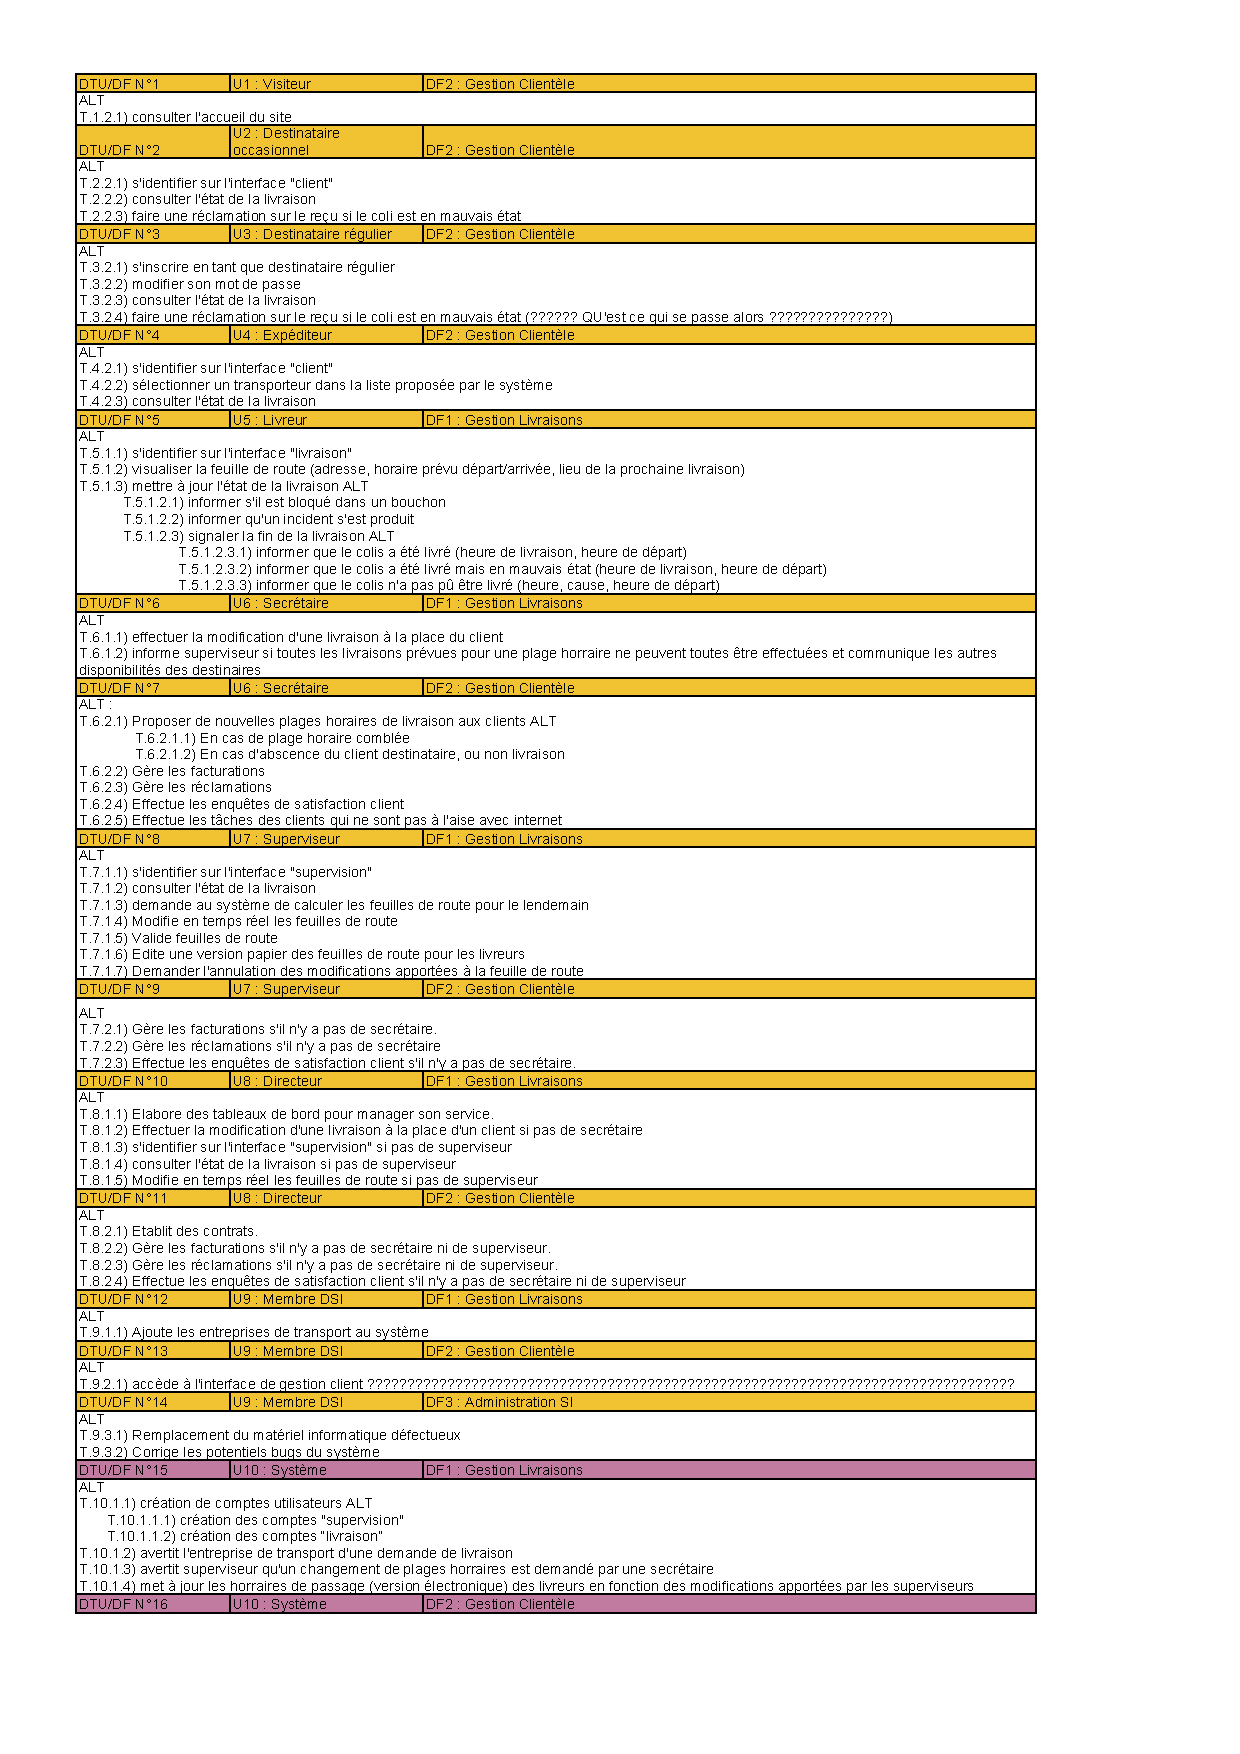
\includegraphics[scale = 0.8]{images/DTUDF.pdf}


%------------------DC-IHM------------------------%

\chapter{Description Conceptuelle de l'IHM}


\section{Dossier d'Initialisation de la Conception de l'IHM}

\subsection{Charte graphique et Guide de style utilisé : }

Nous allons utiliser les deux documents qui nous ont été fournis par la COURLY, et qui sont “charte$\_$graphique$\_$COURLY” pour la charte graphique, et “guide$\_$style$\_$COURLY” pour le guide de style. Ainsi, nous respecterons l’aspect générale de l’application ayant été définie par le client.

\subsection{Ensemble des métaphores : }

\paragraph{Superviseur :}
~~\\
Le superviseur demande au système de calculer les feuilles de routes pour les livraisons du lendemain.\\
Le superviseur modifie la feuille de route en cas de livraisons impossible.\\
Le superviseur peut modifier interactivement les feuilles de route.\\
Le superviseur peut demander une mise à jour des horaires de passage au système.\\
Le superviseur voit les livraisons pour lesquelles la plage horaire ne respecte plus celle demandée par le client.\\
Le superviseur peut annuler les modifications apportées aux feuilles de route.\\
Le superviseur valide des feuilles de route.\\
Le superviseur édite une version papier.\\
Le superviseur observe l’état des livraisons en cours. \\
Le superviseur regarde en détail les informations concernant une livraison (effectuée ou non).\\
Le superviseur modifie la feuille de route d’un livreur (suppression d’une livraison, interversion de l’ordre de deux livraisons, ...).\\
Le superviseur demande au système de re-calculer les feuilles de routes pour les livraisons du lendemain.\\

\paragraph{Livreur :}
~~\\
Le livreur reçoit une version papier de sa feuille de route de la journée.\\
Le livreur visualise sa feuille de route pour la journée.\\
Le livreur visualise les informations détaillées d’une livraison à effectuer dans la journée (l’adresse de livraison, l’heure prévue d’arrivée à cette adresse, l’heure prévue de départ de cette adresse pour le prochain lieu de livraison, les coordonnées d’une personne à contacter en cas de problème).\\
Le livreur peut signaler s’il est bloqué dans un embouteillage.\\
Le livreur peut indiquer qu’il a effectué la livraison et remplir les informations concernant celle-ci (heure de livraison, heure de départ, livraison effectuée ou non - et dans ce dernier cas la cause).\\

\paragraph{Secrétaire :}
~~\\
La secrétaire contact les clients qui possèdent une livraison impossible pour leur proposer une nouvelle plage horaire.\\
La secrétaire informe le superviseur quand il y a des livraisons impossibles.\\

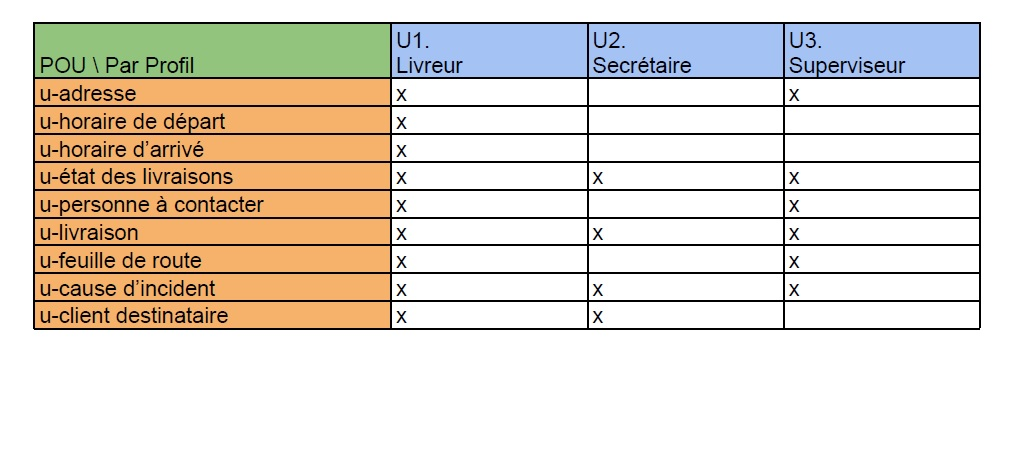
\includegraphics[scale = 0.5]{images/DICIHM.jpg}

\section{Modèle Structurel de l'IHM}

\subsection{Livreur : }
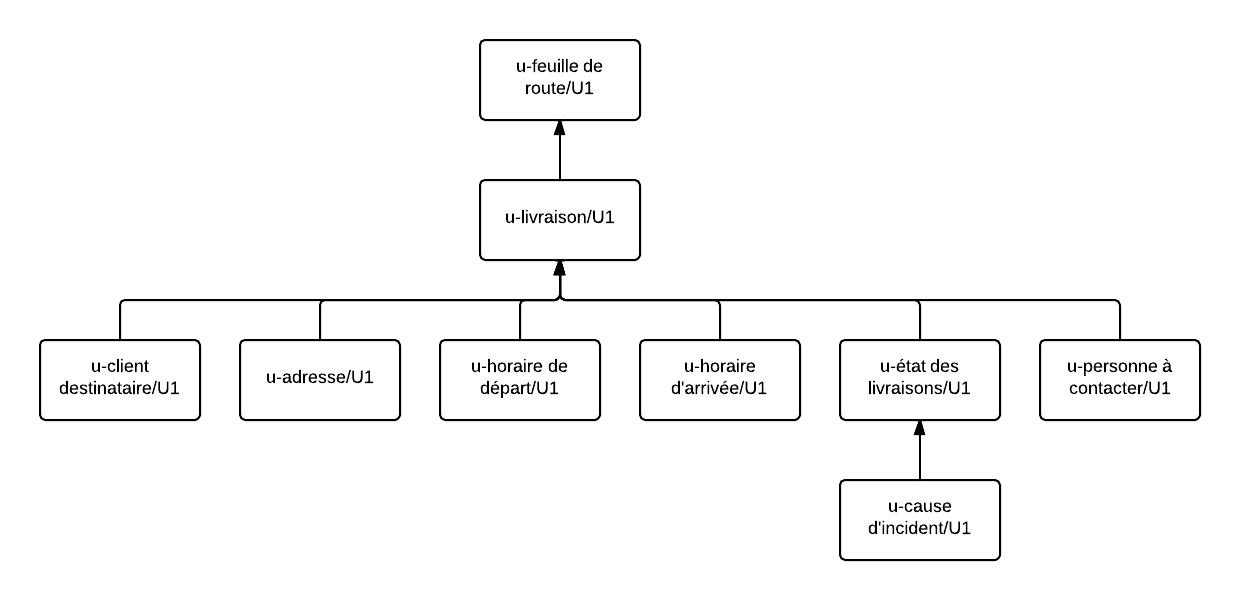
\includegraphics[scale = 0.33]{images/MSIHM-U1.jpeg}

\subsection{Secrétaire : }
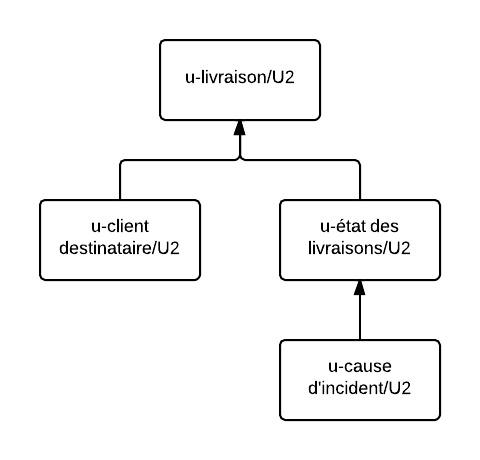
\includegraphics[scale = 0.4]{images/MSIHM-U2.jpeg}

\subsection{Superviseur  : }
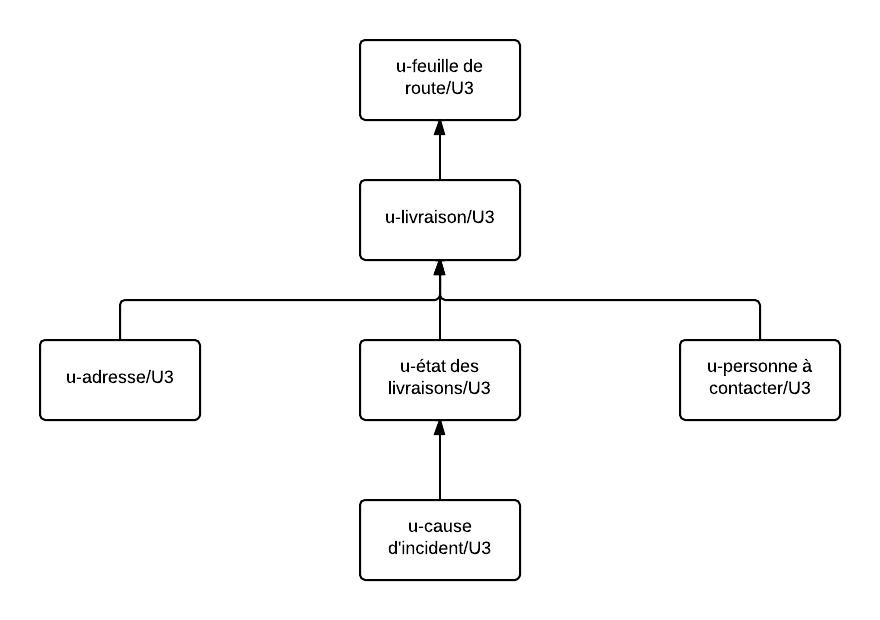
\includegraphics[scale = 0.4]{images/MSIHM-U3.jpeg}

\section{Description détaillée des Principaux Objets Utilisateurs}

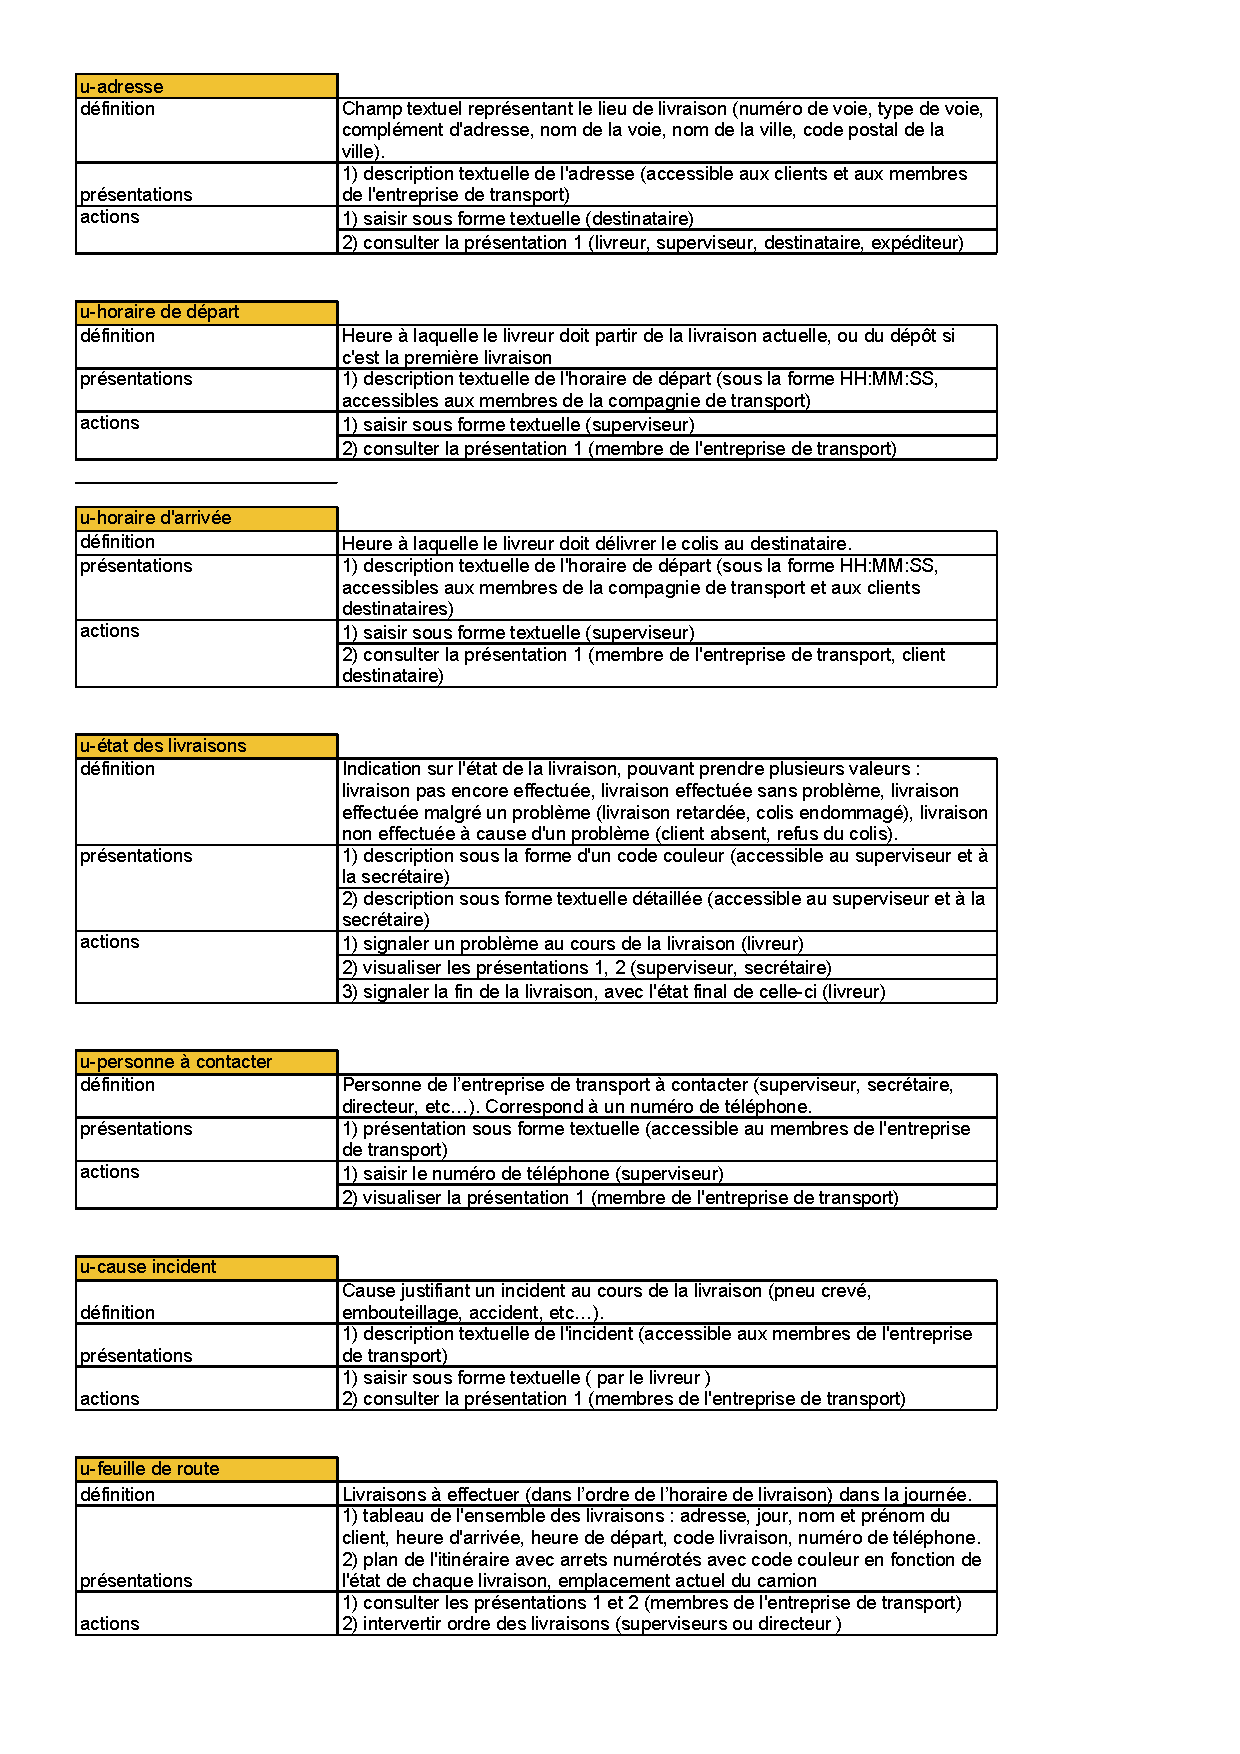
\includegraphics[scale = 0.8, page = 1]{images/DPOU.pdf} 

\paragraph{}

\includegraphics[scale = 0.8, page = 2]{images/DPOU.pdf}

%------------------DS-IHM------------------------%

\chapter{Description de la Sémantique de l'IHM}


\section{Planification Hiérarchique de la Tâche Utilisateur Approfondie}

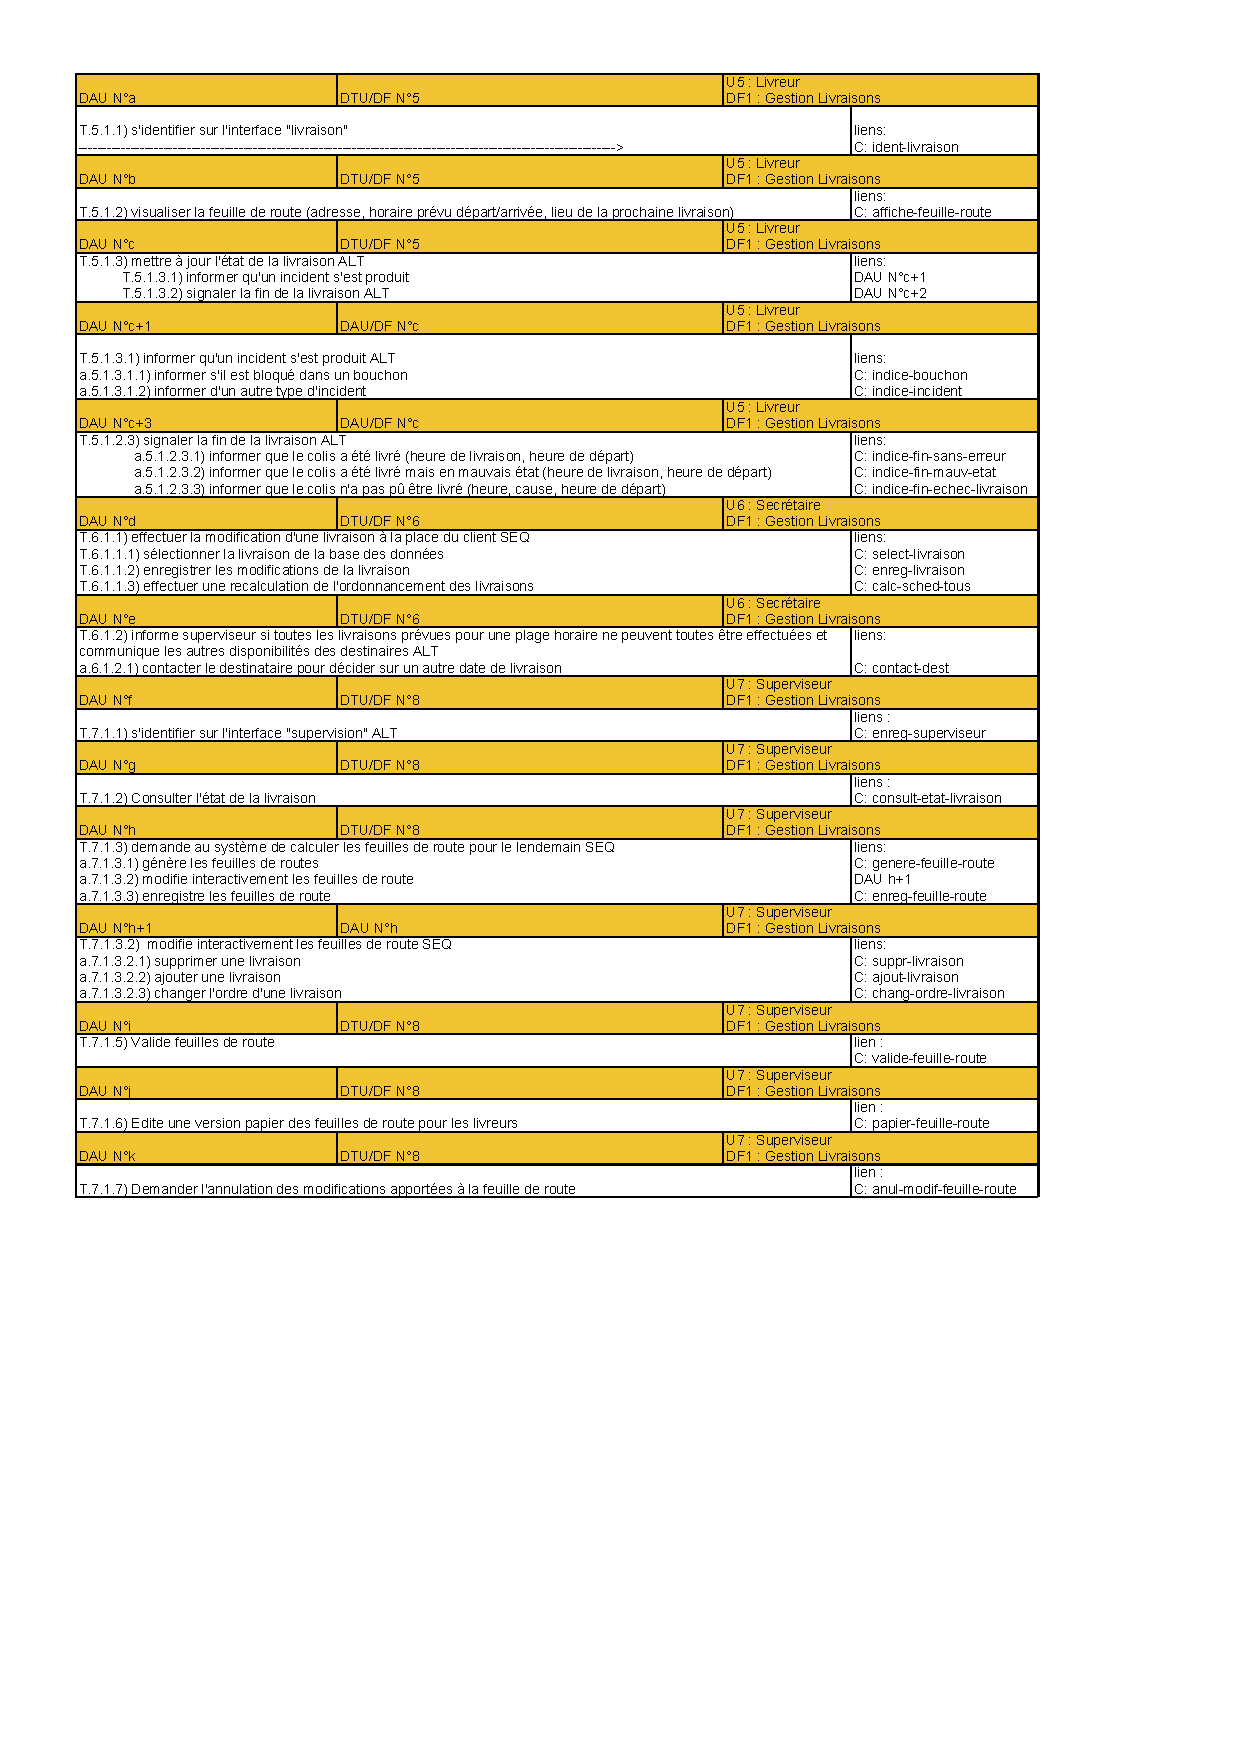
\includegraphics[scale = 0.7]{images/DAU.pdf}

\section{Table des Commandes par Utilisateurs}

\section{Table des Utilisateurs par Commande}

\section{Description des COMmandes}

%-----------------DSy-IHM------------------------%

\chapter{Description Syntaxique de l'IHM}




%------------------DL-IHM------------------------%

\chapter{Description Lexicale de l'IHM}


\begin{appendices}


\chapter{Glossaire}

\end{appendices}

\end{document}
